% Generated by records_reorg.py assemble (records-reorg/); edit the data and re-run, not this file.
\subsection{Earlier OmniFold studies and the practices applied here}\label{recsec:intro-omnifold}

% Compression rewrite (DECISION-20261119c; REWRITE-RULES-20261119.md rule 5; the director's Part 1 rulings, 2026-11-19): text the
% director-helper-3 lane moved verbatim out of the posted note, one move-manifest row per passage (H3-048..H3-050 in
% history-cuts/move-manifest-h3-20261117.tsv). References into the note resolve through main_note.aux (xr). Only passages
% without a citation moved: the note keeps every prior-work citation in its introduction (the director's ruling).
% [records reorg] former heading: \section{Introduction detail moved from the note}
% [records reorg, not printed] This section holds supporting detail that the compressed introduction no longer prints, as the note printed it.

\paragraph{Practices of the cross-experiment guide applied here.}
% [records reorg] former heading: \subsection{Practices of the cross-experiment guide applied here (from Part 1, prior OmniFold applications)}
% From sec_intro.tex (draft e5c56bcc2 lineage), after "Ref. Canelli:2025guide collects these and other applications and distills cross-experiment practice."
Three of the practices it audits are applied here: the ensemble-mean cross-check of the central value and the bootstrap statistical covariance (\S\ref{sec:uq-boot}), and the joint-perturbation (unified-throw) check, used in the five-axis covariance (\S\ref{sec:uq-combine}).

\paragraph{Findings of the first neutrino OmniFold study.}
% [records reorg] former heading: \subsection{Findings of the first neutrino OmniFold study (from Part 1, Huang et al.)}
% From sec_intro.tex (draft e5c56bcc2 lineage), the sentences after the study's description
Two of its findings bear on neutrino applications. The first is its iteration count, which we do not adopt (\S\ref{sec:method-config}). The second is an ensemble of reweighting trials with different train/test splits that controls the ML stochastic component. We include that component explicitly, as the training-seed variation band (\S\ref{sec:systematics}).
The present work differs from that study in three ways. It unfolds \emph{real} MINERvA data to an absolutely normalized cross section, with a 2D uncertainty budget whose covariance components are all built with the central value's own learner (\S\ref{sec:method-config}). Its gradient-boosted decision-tree (GBDT) learners suit a low-dimensional tabular feature set. It compares the result directly with a published binned measurement of the same data (\S\ref{sec:results}).

\subsection{The published MINERvA measurement, and why unbinned}\label{recsec:intro-measurement}

\paragraph{Further introduction detail.}
% Part 1 compression at depth (the director, 2026-11-20; DECISION-20261120a item 5), director-helper-3: uncited sentences
% moved verbatim from sec_intro.tex (H3-P1C-*); every prior-work citation stays in the note (the director's Part 1 ruling (b)).
% [records reorg] former heading: \subsection{Further introduction detail (from Part 1, the compression at depth)}

\paragraph{The data and the published measurement.}
% [records reorg] former heading: \paragraph{The data and the published measurement.}
% From sec_intro.tex, paragraph 5
\emph{After, in \S\ref{sec:intro}, the note's ``MINERvA (Main Injector Experiment for $\nu$-A) is a dedicated neutrino--nucleus scattering experiment in Fermilab's NuMI beamline, immediately upstream of the MINOS near detector~\cite{MINERvA:2013zvz}.'' ``During roughly a decade of operation ending in 2019, it recorded high-statistics samples in low-energy and medium-energy (ME) beam configurations~\cite{MINERvA:2016iqn}.''}
It ran in neutrino-dominated (forward horn current, FHC) and antineutrino-dominated modes. The few-GeV regime combines quasielastic, resonant, and deep-inelastic processes that no single model describes well.
% From sec_intro.tex, paragraph 6
% [lead-in, Option B] \emph{After, in \S\ref{sec:intro}, the note's ``The MINERvA ME FHC charged-current (CC) inclusive double-differential cross section in muon transverse and longitudinal momentum, $d^{2}\sigma/(d\pT\,d\pPar)$, was published by Ruterbories \emph{et al.} \cite{MINERvA:2021owq} using D'Agostini iterative Bayesian unfolding (IBU)~\cite{DAgostini:1994fjx} with a binned response matrix.'' ``We reproduce it with \emph{unbinned} OmniFold~\cite{Andreassen:2019cjw, Andreassen:2021zzk}.''}
OmniFold iteratively reweights events using machine-learned likelihood ratios on per-event observables rather than on a fixed histogram binning.

\paragraph{Why unbinned.}
% [records reorg] former heading: \paragraph{Why unbinned.}
% From sec_intro.tex, paragraph 13
% [lead-in, Option B] \emph{After, in \S\ref{sec:intro}, the note's ``First, OmniFold learns event weights in the full observable space and histograms only the final result.'' ``Reported bins can be chosen or refined after unfolding without rerunning it.''}
Background subtraction is unbinned too in the 2D result and its covariance, in the 3D and 4D central values and in the sixteen-cell five-dimensional result (\S\ref{sec:fived16}). These use refined negative-weight subtraction (\S\ref{sec:method-algo}).
% From sec_intro.tex, paragraph 14
% [lead-in, Option B] \emph{After, in \S\ref{sec:intro}, the note's ``Second, additional observables enter as input features, without multiplying response-matrix bins.''}
The available-energy extension (\S\ref{sec:3d}) is built this way; a binned method such as IBU would need a correspondingly larger multidimensional response matrix to include it.
% From sec_intro.tex, paragraph 15
% [lead-in, Option B] \emph{After, in \S\ref{sec:intro}, the note's ``Third, OmniFold regularizes through model capacity and through an iteration count, which it shares with IBU.''}
Comparing the two methods on the same data probes the result's method dependence (\S\ref{sec:results}).
% From sec_intro.tex, paragraph 17
% [lead-in, Option B] \emph{After, in \S\ref{sec:intro}, the note's ``Section~\ref{sec:part-method} gives the data, the simulation and the method, the earlier note's three question parts answer the three questions, and its part on results and validity tabulates each result with its validity.''}
A scalar study with relaxed truth-muon cuts (App.~\ref{sec:fps}) probes an alternative signal definition. App.~\ref{app:devhistory} lists the superseded configurations, changed tests and consequential choices made after results were seen that bear on the released results. For each, it states what had been seen when it was made. The note will be released as a versioned public document with the Zenodo reproduction package (App.~\ref{app:release}).

\subsection{The dimensionality of MINERvA's published measurements}\label{recsec:intro-survey}

\paragraph{Detail.}
% Records document: detail moved verbatim from the posted note in the 2026-11 compression (DECISION-20261119c-joseph-note-compression-outline.md
% item 3; move-manifest-je JE-10, JE-12). It holds two kinds of text: the history of stopped tests and superseded comparisons
% (class H, the director's App. E ruling), and current detail of later reporting-only studies that the compressed note states
% in short form. Neither is a struck value; app_history.tex keeps those.
% [records reorg] former heading: \section{Detail moved from the note in the compression}
\label{app:compression-records}

\paragraph{The MINERvA measurement-dimensionality survey.}
% Moved verbatim from the note in the compression (LM; move-manifest-je JE-14): the dimensionality survey (app_landscape.tex, App. E's
% parked appendix) and its figure (sec_3d.tex, fig:landscape), together, so every \ref between them resolves here. limitation-resolver's OK for
% the sec_3d.tex edits, 2026-11-19.
% [records reorg] former heading: \subsection{The MINERvA measurement-dimensionality survey}
\label{app:landscape}
The survey behind Fig.~\ref{fig:landscape} lists MINERvA differential cross-section measurements through the listed 2025 entries, with references and dimensionality: the number of kinematic variables unfolded simultaneously in each analysis's main differential result. The survey is nonexhaustive through 2026; recent additions follow.
{\small
\begin{longtable}{@{}clcl@{}}
  \caption{MINERvA differential cross-section survey used for the landscape figure, with the dimensionality
  (Dim.) defined in the text. Channels: CC-inclusive (incl.),
  CCQE/QE-like incl.\ transverse kinematic imbalance (QE), pion production CC
  and coherent ($\pi$), deep-inelastic / kaon (DIS), electron-neutrino
  ($\nu_e$), nuclear-target ratio (ratio).}
  \label{tab:landscape}\\
  \toprule
  Year & Channel; observables & Dim. & Ref. \\
  \midrule
  \endfirsthead
  \toprule
  Year & Channel; observables & Dim. & Ref. \\
  \midrule
  \endhead
  \midrule \multicolumn{4}{r}{\emph{continued\ldots}}\\ \endfoot
  \bottomrule
  \endlastfoot
  2013 & QE; $\nu_\mu$ CCQE $\pT,\pPar$            & 2 & \cite{MINERvA:2013qe} \\
  2013 & QE; $\bar\nu_\mu$ CCQE $\pT,\pPar$        & 2 & \cite{MINERvA:2013qebar} \\
  2014 & ratio; CC on C/Fe/Pb to CH               & 1 & \cite{MINERvA:2014ratio} \\
  2014 & $\pi$; coherent $\pi^\pm$ (total \& diff.) & 1 & \cite{MINERvA:2014coh} \\
  2015 & $\pi$; CC $1\pi^+$ ($T_\pi$, $\theta_\pi$) & 1 & \cite{MINERvA:2015ydy} \\
  2015 & QE; $\mu$+p final states                 & 1 & \cite{MINERvA:2015mup} \\
  2015 & $\pi$; $\bar\nu_\mu$ single $\pi^0$       & 1 & \cite{MINERvA:2015pi0} \\
  2016 & $\nu_e$; CCQE-like on CH                  & 2 & \cite{MINERvA:2016nueqe} \\
  2016 & $\pi$; $\nu_\mu/\bar\nu_\mu$ pion prod.   & 2 & \cite{MINERvA:2016pion} \\
  2016 & DIS; partonic nuclear effects            & 2 & \cite{MINERvA:2016dis} \\
  2016 & DIS; CC $K^+$ production                  & 1 & \cite{MINERvA:2016kaon} \\
  2017 & $\pi$; CC single $\pi^0$                  & 2 & \cite{MINERvA:2017pi0} \\
  2017 & QE; nuclear-dependence (multi-target)     & 1 & \cite{MINERvA:2017Adep} \\
  2018 & QE; $\bar\nu_\mu$ QE-like $\pT,\pPar$     & 2 & \cite{MINERvA:2018hba} \\
  2018 & QE; $\mu$-p mesonless TKI                 & 2 & \cite{MINERvA:2018tcb} \\
  2018 & $\pi$; coherent $\pi^\pm$ on C            & 2 & \cite{MINERvA:2018coh} \\
  2019 & QE; quasielastic-like $\nu_\mu$           & 2 & \cite{MINERvA:2019qe} \\
  2019 & $\pi$; $\bar\nu_\mu$ single $\pi^-$       & 2 & \cite{MINERvA:2019pim} \\
  2020 & incl.; CC-incl $\langle E_\nu\rangle\!\sim\!3.5$ GeV $\pT,\pPar$ & 2 & \cite{MINERvA:2020jwd} \\
  2020 & QE; nuclear binding \& TKI               & 2 & \cite{MINERvA:2020cgh} \\
  2020 & QE; high-statistics QE-like              & 2 & \cite{MINERvA:2020qehs} \\
  2020 & $\pi$; CC $\pi^0$ nuclear effects        & 1 & \cite{MINERvA:2020pi0} \\
  2021 & incl.; CC-incl $\langle E_\nu\rangle\!\sim\!6$ GeV $\pT,\pPar$ \textbf{(target)} & 2 & \cite{MINERvA:2021owq} \\
  2022 & QE; QE-like $\pT,\pPar,\Sigma T_p$ (triple-diff.) & 3 & \cite{MINERvA:2022qelike3d} \\
  2022 & incl.; CC-incl low-$q_{3}$ ($\Eavail$, $q_{3}$) & 2 & \cite{MINERvA:2022incl} \\
  2023 & $\pi$; CC $1\pi^+$ (multi-target)        & 2 & \cite{MINERvA:2023ccpi} \\
  2023 & $\pi$; coherent $\pi^+$ (multi-target)   & 1 & \cite{MINERvA:2023coh} \\
  2023 & QE; $\bar\nu_\mu$ multi-neutron low-$\Eavail$ & 1 & \cite{MINERvA:2023lowEavail} \\
  2024 & $\nu_e$; low-$Q^2$ ($\Eavail$, $\pT$)    & 2 & \cite{MINERvA:2023avz} \\
  2025 & QE; $A$-dependence TKI (multi-target)    & 2 & \cite{MINERvA:2025tki} \\
  \midrule
  2026 & \textbf{this work}; unbinned $\pT,\pPar$            & 2 & --- \\
  2026 & \textbf{this work}; unbinned $\pT,\pPar,\Eavail$    & \textbf{3} & --- \\
  2026 & \textbf{this work}; unbinned $\pT,\pPar,\Eavail,q_{3}$ & \textbf{4} & --- \\
  2026 & \textbf{this work}; unbinned $\pT,\pPar,\Eavail,q_{3},W$ (illustrative output) & \textbf{5} & --- \\
\end{longtable}
}

\paragraph{Additional recent measurements.}
% [records reorg] former heading: \paragraph{Additional recent measurements.}
 The low-/medium-energy comparison of quasielastic-like cross sections unfolds three variables simultaneously, $\pT$, $\pPar$, and available recoil energy \cite{MINERvA:2026qeleme}; it has the dimensionality of our three-dimensional result, with a different signal from our inclusive one. The shallow-inelastic measurement reports one-dimensional neutrino and antineutrino cross sections \cite{MINERvA:2026sis}. Other measurements report single-differential charged-pion production down to zero pion kinetic energy \cite{MINERvA:2026pion} and inclusive antineutrino cross sections versus $\pT$ on several targets~\cite{MINERvA:2026antinu}. These channel-specific additions are not plotted in Fig.~\ref{fig:landscape}.
\begin{figure}[H]
  \centering
  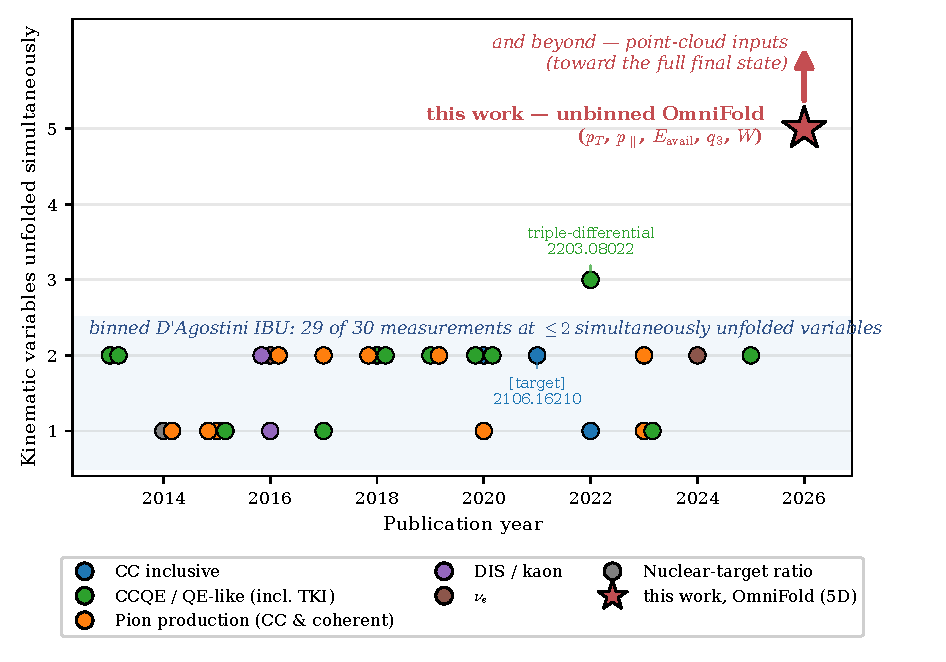
\includegraphics[width=\textwidth]{minerva_unfolding_landscape}
  \caption[Survey of MINERvA differential measurements]{This work unfolds five recorded CC-inclusive high-level observables without binning. Earlier results use binned unfolding, including a triple-differential quasielastic-like measurement. The survey shows MINERvA differential measurements by number of simultaneously unfolded kinematic variables, by year, colored by channel (a double-differential $d^{2}\sigma/dx\,dy$ counts as two). Sources: the MINERvA data-release page and cited publications. The inventory runs through 2025, with newer measurements in App.~\ref{app:landscape}. Classification uses headline differential results, excluding flux, reconstruction, generator-tuning and total-only entries.}
  \label{fig:landscape}
\end{figure}
